\documentclass{ctexart}
\usepackage[a4paper, margin=1in]{geometry}  % 设置边距
\usepackage{graphicx}  % 引入graphicx宏包
\usepackage{tikz}
% \usetikzlibrary{intersections}
% \usetikzlibrary {arrows.meta}
% \usetikzlibrary{angles,quotes}

\usetikzlibrary{decorations.pathmorphing,backgrounds,fit}
% \usepackage{xcolor} % 确保引入了 xcolor 宏包
\usetikzlibrary {arrows.meta,petri,positioning}
\begin{document}


    \begin{figure}[h]  % 浮动环境
        \centering  % 图片居中
        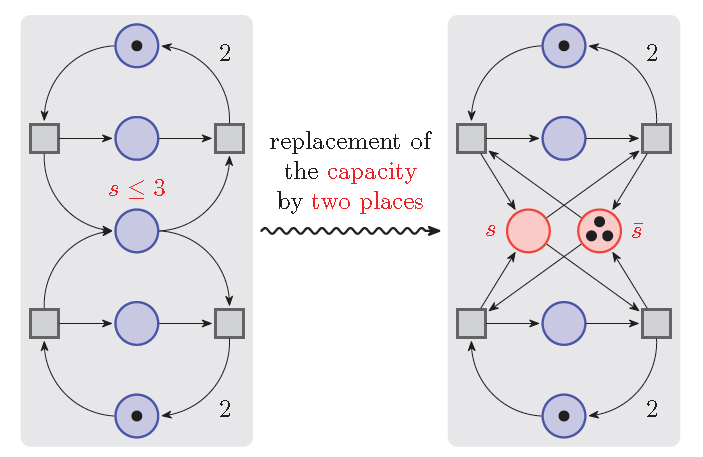
\includegraphics[width=\textwidth]{3-APetriNetForHagen.png}  % 插入图片(无需扩展名)
        \caption{这是一个示例图片}  % 图片说明
        \label{fig:example}  % 引用标签
    \end{figure}
    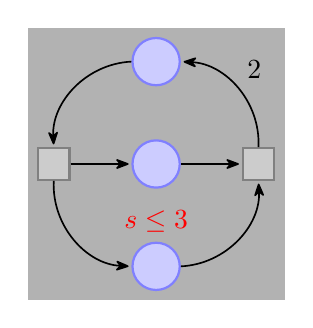
\begin{tikzpicture}
        [
            node distance=1.3cm,
            on grid,
            >={Stealth[round]},
            bend angle=45, 
            auto,
            pre/.style={<-,shorten <=1pt,,semithick},
            post/.style={->,shorten >= 1pt,>={Stealth[round]},semithick},
            every label/.style={red},
            place/.style={circle,draw=blue!50,fill=blue!20,thick,inner sep=0pt,minimum size=6mm},
            transition/.style={rectangle,draw=black!50,fill=black!20,thick,inner sep=0pt,minimum size=4mm}
        ]

        \node[place] (waiting) {};
        \node[place] (critical) [below=of waiting] {};
        \node[place] (semaphore) [below=of critical,label=above:$s \le 3$] {};
        \node[transition] (leave critical) [right=of critical] {}
            edge [pre]  (critical) 
            edge [post,bend right] node[swap] {2} (waiting)
            edge [pre,bend left] (semaphore);
        \node[transition] (enter critical) [left=of critical] {}
            edge [post] (critical)
            edge [pre,bend left] (waiting)
            edge [post,bend right] (semaphore);
        
        \begin{scope}[on background layer]
            \node [fill=black!30,fit=(waiting) (critical) (semaphore) (leave critical) (enter critical)] {};
        \end{scope}
    \end{tikzpicture}

    \tikz \node [circle,draw,label=60:$ 60^\circ $,label=below:$ -90^ \circ $] {my circle};

    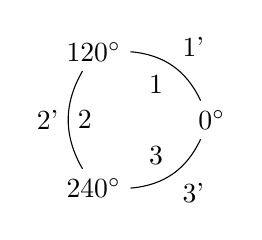
\begin{tikzpicture}[auto,bend right]
        \node (a) at (0:1) {$0^\circ$};
        \node (b) at (120:1) {$120^\circ$};
        \node (c) at (240:1) {$240^\circ$};

        \draw   (a) to node {1} node[swap] {1'} (b)
                (b) to node {2} node[swap] {2'} (c)
                (c) to node {3} node[swap] {3'} (a);
    \end{tikzpicture}
    
    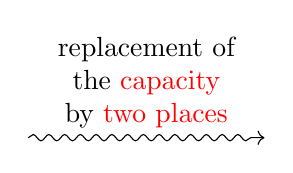
\begin{tikzpicture}
        \draw [->,decorate,decoration={snake,amplitude=.4mm,segment length=2mm,post length=1mm}] (0,0) -- (3,0) node[above,align=center,midway] {
            replacement of \\
            the \textcolor{red}{capacity}   \\
            by \textcolor{red}{two places}
        };
    \end{tikzpicture}

    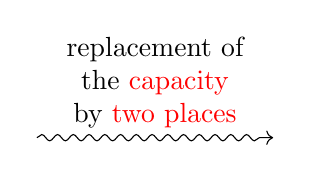
\begin{tikzpicture}
        \draw [->,decorate,decoration={snake,amplitude=.4mm,segment length=2mm,post length=1mm}] (0,0) -- (3,0) node[above,text width=3cm,align = center,midway] {
            replacement of the \textcolor{red}{capacity}  
            by \textcolor{red}{two places}
        };
    \end{tikzpicture}


    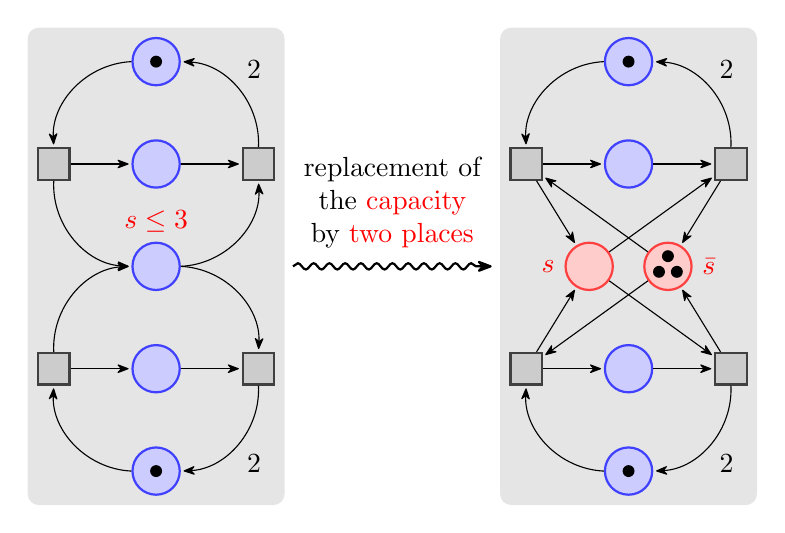
\begin{tikzpicture}
        [node distance=1.3cm,on grid,>={Stealth[round]},bend angle=45,auto,
        every place/.style= {minimum size=6mm,thick,draw=blue!75,fill=blue!20},
        every transition/.style={thick,draw=black!75,fill=black!20},
        red place/.style={place,draw=red!75,fill=red!20},
        every label/.style={red}]

   

        \node [place,tokens=1] (w1) {};
        \node [place] (c1) [below=of w1] {};      
        \node [place] (s) [below=of c1,label=above:$s\le 3$] {};
        \node [place] (c2) [below=of s] {};
        \node [place,tokens=1] (w2) [below=of c2] {};

        \node [transition] (e1) [left=of c1] {}
            edge [pre,bend left] (w1)
            edge [post,bend right] (s)
            edge [post] (c1);
        \node [transition] (e2) [left=of c2] {}
            edge [pre,bend right] (w2)
            edge [post,bend left] (s)
            edge [post] (c2);
        \node [transition] (l1) [right=of c1] {}
            edge [pre] (c1)
            edge [pre,bend left] (s)
            edge [post,bend right] node[swap] {2} (w1);
        \node [transition] (l2) [right=of c2] {}
            edge [pre] (c2)
            edge [pre,bend right] (s)
            edge [post,bend left] node {2} (w2);
        \begin{scope}[xshift=6cm]
            \node [place,tokens=1] (w1') {};
            \node [place] (c1') [below=of w1'] {};
            \node [red place] (s1') [below=of c1',xshift=-5mm]
                [label=left:$s$] {};
            \node [red place,tokens=3] (s2') [below=of c1',xshift=5mm]
                [label=right:$\bar s$] {};
            \node [place] (c2') [below=of s1',xshift=5mm] {};
            \node [place,tokens=1] (w2') [below=of c2'] {};
            \node [transition] (e1') [left=of c1'] {}
                edge [pre,bend left] (w1')
                edge [post] (s1')
                edge [pre] (s2')
                edge [post] (c1');
            \node [transition] (e2') [left=of c2'] {}
                edge [pre,bend right] (w2')
                edge [post] (s1')
                edge [pre] (s2')
                edge [post] (c2');
            \node [transition] (l1') [right=of c1'] {}
                edge [pre] (c1')
                edge [pre] (s1')
                edge [post] (s2')
                edge [post,bend right] node[swap] {2} (w1');
            \node [transition] (l2') [right=of c2'] {}
                edge [pre] (c2')
                edge [pre] (s1')
                edge [post] (s2')
                edge [post,bend left] node {2} (w2');
        \end{scope}
        
        \begin{scope}[on background layer]
            \node (r1) [fill=black!10,rounded corners,fit=(w1)(w2)(e1)(e2)(l1)(l2)] {};
            \node (r2) [fill=black!10,rounded corners,fit=(w1')(w2')(e1')(e2')(l1')(l2')] {};
        \end{scope}

        \draw [shorten >=1mm,->,thick,decorate,
            decoration={snake,amplitude=.4mm,segment length=2mm,
            pre=moveto,pre length=1mm,post length=2mm}]
            (r1) -- (r2) node [above=1mm,midway,text width=3cm,align=center]
            {replacement of the \textcolor{red}{capacity} by \textcolor{red}{two places}};
    \end{tikzpicture}
\end{document}